\documentclass[a4paper,11pt]{article}
\input{/home/tof/Documents/Cozy/latex-include/preambule_lua.tex}
\newcommand{\showprof}{show them}  % comment this line if you don't want to see todo environment
\fancyhead[L]{Exercices graphes représentation}
\newdate{madate}{10}{09}{2020}
%\fancyhead[R]{\displaydate{madate}} %\today
%\fancyhead[R]{Seconde - SNT}
%\fancyhead[R]{Première - NSI}
\fancyhead[R]{Terminale - NSI}
\fancyfoot[L]{~\\Christophe Viroulaud}
\AtEndDocument{\label{lastpage}}
\fancyfoot[C]{\textbf{Page \thepage/\pageref{lastpage}}}
\fancyfoot[R]{\includegraphics[width=2cm,align=t]{/home/tof/Documents/Cozy/latex-include/cc.png}}
\usepackage{tikz}
\begin{document}
\begin{Form}
Dans les exercices suivants, nous pourrons tester les méthodes sur le graphe \ref{graphe}.
\begin{center}
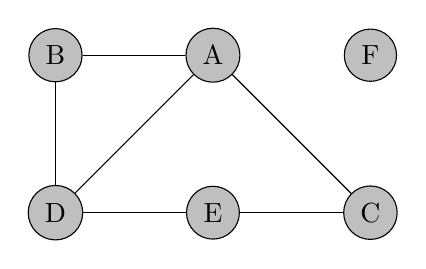
\begin{tikzpicture}
\node[draw,circle,fill=gray!50] (A)at(0,2) {A};
\node[draw,circle,fill=gray!50] (B)at(-2,2) {B};
\node[draw,circle,fill=gray!50] (C)at(2,0) {C};
\node[draw,circle,fill=gray!50] (D)at(-2,0) {D};
\node[draw,circle,fill=gray!50] (E)at(0,0) {E};
\node[draw,circle,fill=gray!50] (F)at(2,2) {F};
\draw[-,>=latex] (A) -- (B);
\draw[-,>=latex] (A) -- (C);
\draw[-,>=latex] (A) -- (D);
\draw[-,>=latex] (D) -- (B);
\draw[-,>=latex] (D) -- (E);
\draw[-,>=latex] (C) -- (E);
\end{tikzpicture}
\captionof{figure}{Graphe pour tester les méthodes}
\label{graphe}
\end{center}
\begin{exo}
\begin{itemize}
\item Construire la matrice d'adjacence (sur papier puis sur machine) du graphe figure \ref{graphe}.
\item Construire le dictionnaire d'adjacence du graphe figure \ref{graphe}.
\end{itemize}
\end{exo}
\begin{exo}
Dessiner tous les graphes non orientés ayant exactement trois sommets.
\end{exo}
\begin{exo}
Ajouter à la classe \emph{Graphe} la méthode \textbf{afficher(self)$\;\rightarrow\;$str} qui retourne une chaîne de caractère de la forme:
\begin{itemize}
\item A \{ B C D \}
\item B \{ A D \}
\item ...
\end{itemize}
\end{exo}
\begin{exo}
Ajouter à la classe \emph{Graphe} la méthode \textbf{nb\_sommets(self)$\;\rightarrow\;$int} qui renvoie l'ordre de ce graphe.
\end{exo}
\begin{exo}
Ajouter à la classe \emph{Graphe} la méthode \textbf{degre(self, sommet: str)$\;\rightarrow\;$int} qui renvoie le degré de \emph{sommet}.
\end{exo}
\begin{exo}
\begin{enumerate}
\item Dans la représentation du graphe, il faut remarquer que chaque arête est comptée deux fois. Quelle relation peut-on alors écrire entre le nombre d'arêtes et la somme totale des degrés?
\item Ajouter à la classe \emph{Graphe} la méthode \textbf{nb\_aretes(self)$\;\rightarrow\;$int} qui renvoie le nombre total d'arêtes.
\end{enumerate}
\end{exo}
\begin{exo}
Ajouter à la classe \emph{Graphe} la méthode \textbf{supprimer(self, sommet: str)$\;\rightarrow\;$None} qui retire le \emph{sommet} du graphe (ainsi que les arêtes le concernant).
\end{exo}
\end{Form}
\end{document}